\documentclass[a4paper,parskip=half]{article} %scrartcl article
\usepackage[utf8]{inputenc}
\usepackage[T1]{fontenc}
\usepackage{amsmath,amssymb,mathtools}
\usepackage{hyperref,cleveref,xcolor}

\usepackage{tikz-cd}
\usepackage[top=1.5cm,bottom=3.2cm,left=2.5cm,right=2.5cm]{geometry}

\newcommand*\id{\operatorname{id}}

\newcommand*\spec[1]{\textcolor{blue}{\texttt{#1}}}
\newcommand{\delete}[1]{}


\author{Franz Brauße  \and
	Zurab Khasidashvili \and
	Konstantin Korovin}

\begin{document}

\section{Assumptions}
Let $f_1,\ldots,f_n$ be \emph{features} and let
the index set $\{1,\ldots,n\}$ be partitioned into the three sets $K,I$ and $R$.
Let $V_i%\subseteq\Sigma^*
$ be the set of valid values
in any data set described by the feature $f_i$ for $i=1,\ldots,n$.
For every feature $f_i$ there is an associated \emph{embedding} $e_i:V_i\to A_i$
into a subset $A_i$ of Euclidean space $\mathbb R^{n_i}$ and
there is an associated \emph{label} $\ell_i\in\Sigma^*$.
All labels are pairwise different.
The \emph{approximator} $\mathcal N$ is a function
$\mathcal K\times\mathcal I\to\mathcal R$ where
the sets $\mathcal K,\mathcal I$ and $\mathcal R$ are the cartesian products of
$\mathbb R^{n_i}$ for $i$ in $K,I$ and $R$, respectively.

These assumptions are satisfied by any finite combination of features of types
depicted in \cref{tab:features}.
Please note that the attribution of `discrete' or `continuous' refers to the
concept of discreteness of topological spaces when $A_i$ is seen as a metric
space with the standard Euclidean distance $d_2:(x,y)\mapsto\Vert x-y\Vert_2$.
%except where noted differently.
%The actual predicates over the corresponding spaces $A_i$, affect either
%the topology, continuity/computability of the mapping $e_i$ or whether the
%predicate is computable over $V_i$.
$\mathbb F_{64}$ refers to IEEE-754 \texttt{binary64} double-precision
floating point numbers.


\begin{table}[h]
\centering\small
\def\arraystretch{1.2}
\begin{tabular}{p{8.8em}|p{16em}|p{15.3em}}
Set $V$ of values & Attributes of $V$ and $e$ & Example `embedding' $e$
%& Metric
% & ... space $A\subseteq\mathbb R^n$
\\ \hline\hline
$\{x_1,\ldots,x_n\}$ \newline (finite set)
& unordered, discrete, finite, injective
& $x_i\mapsto(\underbrace{0,\ldots,0}_{\mathclap{i-1~\text{times}}},1,0,\ldots,0)\in\{0,1\}^n$
%& $d_2$
%& VS $(\{0,1\}^n,\oplus)$
\\ \hline
$\{x_0,\ldots,x_{b-1}\}^*$ \newline (finite strings)
& \raggedright unordered, discrete, bijective
& %$(x_{j_n},\ldots,x_{j_0})\mapsto\sum_{i=0}^n j_i\cdot b^i$
  %\raggedright
  $(x_{j_n},\ldots,x_{j_1})\mapsto\langle j_n,\ldots,j_1\rangle$, \newline
  for $b$-ary encoding $\langle\cdots\rangle$ on $\mathbb N$
%& $d_2$
%& $\mathbb N$
\\ \hline\hline
$\mathbb Z$
& \raggedright totally ordered, discrete, bijective %, numerical
& $\id:x\mapsto x\in\mathbb Z$
%& $d_2$
%& R $(\mathbb Z,\leq,+,\cdot)$
\\ \hline
$\mathbb Q,\mathbb A$
& \raggedright totally ordered, continuous, bijective %, numerical
& $\id:x\mapsto x\in\mathbb Q,\mathbb A$ respectively %$(p,q)\mapsto\frac pq\in\mathbb Q$ %or $\operatorname{fl_{nearest}}:\mathbb R\to\mathbb F_{64}\setminus\mathtt{NaN}$
%& $d_2$
%& F $(\mathbb Q,\leq,+,\cdot)$
\\ \hline
%$\mathbb Q$ or algebraic
%& \raggedright totally ordered, discrete, numerical, bijective
%& $\id:x\mapsto x$ %$(p,q)\mapsto\frac pq\in\mathbb Q$ %or $\operatorname{fl_{nearest}}:\mathbb R\to\mathbb F_{64}\setminus\mathtt{NaN}$
%& $(x,y)\mapsto\begin{cases}0&\text{if}~x=y\\1&\text{otherwise}\end{cases}$
%& F $(\mathbb Q,\leq,+,\cdot)$
%\\ \hline
$\mathbb F_{64}\setminus\mathtt{NaN}$
& \raggedright preordered, continuous %, numerical
& $-0.0\mapsto 0$, $x\mapsto x\in\mathbb Q$ otherwise
%& $d_2$
%& F $(\mathbb Q,\leq,+,\cdot)$
\\ \hline
$\mathbb F_{64}\setminus(\mathtt{NaN}\cup\{-0.0\})$
& \raggedright totally ordered, discrete, injective %, numerical
& $x\mapsto x\in\mathbb Q$
\end{tabular}
\caption{%
	Common features types satisfying the assumptions.
	%`VS': vector space, 'R': ring, 'F': field, `$\oplus$': XOR.%
}
\label{tab:features}
\end{table}

\section{Specification file}


This section describes the current format of the specification file
(also referred to as \texttt{.spec}-file or simply \texttt{data.spec}).
A \emph{specification} consists of several fields, such as \spec{version}, \spec{variables}, \spec{alpha}, etc. 
The purpose of these fields is described in the itemized list below. The field \spec{variables} is itself  a list of sets of 
pairs $(k_{ij},v_{ij})$ describing the features $f_1,\ldots,f_n$ as follows.
%
A feature $f_i$ with the identity embedding $e_i:x\mapsto x$ is described by
\begin{description}
\item[\spec{version}] Spec format version. Currently 1.2.
\item[\spec{variables}] Specifies types, ranges, and more, for inputs, knobs, and outputs, as follows:
\begin{itemize}%[align=right]
\item[\spec{label}] $\ell_i$
\item[\spec{interface}]
	$\begin{cases}
		\spec{knob}     & \text{if}~i\in K \\
		\spec{input}    & \text{if}~i\in I~\text{and}~V_i~\text{is infinite} \\
		%\spec{categorical} & \text{if}~i\in I~\text{and}~V_i~\text{is finite} \\
		\spec{output} & \text{if}~i\in R
	\end{cases}$

	%Support for \spec{input} is not fully checked, yet.
\item[\spec{type}]
	$\begin{cases}
		\spec{int}  &\text{if}~A_i=\mathbb Z \\
		\spec{real}  &\text{if}~A_i=\mathbb Q \\
		\spec{set} \,\, (x_1,\ldots,x_n) & \text{if}~i\in I~\text{and}~V_i=\{x_1,\ldots,x_n\}
	\end{cases}$

	Optional when \spec{type} is \spec{output}.
\item[\spec{range}] 
Mandatory field to specify the range for int and real typed variables as a closed interval $[a, b]$. 
Optional for set-typed variables.
\item[\spec{grid}]
	Optionally specifies the candidate grid as a vector $(x_1,\ldots,x_m)$
	with $x_k\in V_i$ for all $k=1,\ldots,m$.
	Only takes effect when \spec{interface} is \spec{knob}.
\item[\spec{rad-abs} or \spec{rad-rel}]
	The maximal absolute or relative distance of $y\in A_i$ from point $x\in A_i$
	in order to consider $y$ to be inside the region around $x$.
	Only required for $i\in K$.
	A region around $x$ is considered to one of the the following sets.
	\begin{center}
	\begin{tabular}{ll}
		$\{y\in A_i:x-d\leq y<x+d\}$ &
			if \spec{rad-abs} is $d$ and \spec{range} is \spec{int} \\
		$\{y\in A_i:\Vert x-y\Vert\leq d\}$ &
			if \spec{rad-abs} is $d$ and \spec{range} is \spec{real} \\
		$\{y\in A_i:\Vert x-y\Vert\leq\max(1,|x|\cdot d)\}$ &
			if \spec{rad-rel} is $d$ and \spec{range} is \spec{real} \\
	\end{tabular}
	\end{center}
\end{itemize}
\item[\spec{alpha}] Constraints on inputs and knobs, in addition to whose defined through the \spec{range} field for inputs and knobs.
\item[\spec{eta}] Constraints on knobs, in addition to whose defined through the \spec{range} and \spec{grid} field for knobs.
\item[\spec{beta}] Constraints on inputs,  knobs and outputs.
\item[\spec{queries}] Queries for which SMLP searches for a stable witness in mode \emph{query}.
\item[\spec{assertions}] Assertions to be verified on the model in \emph{verify} mode for the specified values of knobs, and to be guaranteed in mode \emph{synthesize} in the stability region computed during synthesis.
\item[\spec{objectives}] Optimization objectives in \emph{optimize} and \emph{optsyn} (optimized synthesis) modes.
\end{description}

For convenience, the spec file and its fields are written as dictionaries in JSON format.
Any parts of this specification language marked in \spec{blue} are subject to change.

\subsection{Examples}

Figure~\cref{fig:spec} displays an example spec file.

\delete{
\begin{center}
\begin{tabular}{rcccc}
	& $\ell$ & $V$ & $A$ & Index partition \\ \hline
	\ref{it:Timing} & Timing & $\mathbb Z$ & $\mathbb Z$ & $I$ \\
	\ref{it:Byte} & Byte & $\{0,1,\ldots,7\}$ & $\{0,1\}^8$ & $I$ \\
	\ref{it:gain} & TXEQ\_GAIN & $\mathbb Z$ & $\mathbb Q$ & $K$ \\
	\ref{it:delta} & delta & $\mathbb Q$ & $\mathbb Q$ or $\mathbb R$ & $R$
\end{tabular}
\end{center}
\begin{enumerate}
\item\label{it:Timing}
	{\footnotesize\verb!{ "label": "Timing",    "type": "input",    "range": "int", "rad-abs": 5 }!}
\item\label{it:Byte}
	{\footnotesize\verb!{ "label": "Byte",      "type": "categorical", "range": [0,1,2,3,4,5,6,7] }!}
\item\label{it:gain}
	{\footnotesize\verb!{ "label": "TXEQ_GAIN", "type": "knob",     "range": "float", "safe": [1,2,3], "rad-rel": 0.1 }!}
\item\label{it:delta}
	{\footnotesize\verb!{ "label": "delta",     "type": "response" }!}
\end{enumerate}
}

\begin{figure}%[tp]
%\scriptsize
%\tiny
\small
\begin{verbatim}
{
  "version": "1.2",
  "variables": [
    {"label":"y1", "interface":"output", "type":"real"},
    {"label":"y2", "interface":"output", "type":"real"},
    {"label":"x1", "interface":"input", "type":"real", "range":[0,10]},
    {"label":"x2", "interface":"input", "type":"int", "range":[-1,1]},
    {"label":"p1", "interface":"knob", "type":"real", "range":[0,10], "rad-rel":0.1, "grid":[2,4,7]},
    {"label":"p2", "interface":"knob", "type":"int", "range":[3,7], "rad-abs":0.2}
  ],
  "alpha": "p2<5 and x1==10 and x2<12",
  "beta": "y1>=4 and y2>=8",
  "eta": "p1==4 or (p1==8 and p2 > 3)",
  "assertions": {
    "assert1": "(y2**3+p2)/2>6",
    "assert2": "y1>=0",
    "assert3": "y2>0"
  },
  "objectives": {
    "objective1": "(y1+y2)/2",
    "objective2": "y1"
  }
}
\end{verbatim}
\begin{tikzpicture}[remember picture,overlay,shift={(22em,\baselineskip)}]
\node[anchor=south west]{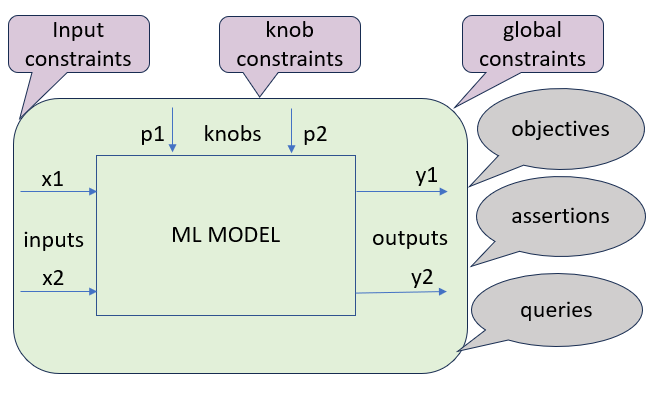
\includegraphics[height=14\baselineskip]{smlp_encoding.PNG}};
\end{tikzpicture}
\vspace*{-1\baselineskip}
\caption{Example of SMLP's format specifying the problem conditions for the displayed model of the system.}
\label{fig:spec}
\end{figure}


\end{document}
